%%%%%%%%%%%%%%%%%%%%%%%%%%%%%%%%%%%%%%%%%%%%%%%%%%%%%%%%%%%%%%%%%%%%%%%%%%%%%%%%
\chapter{Single Image: Statistical Models of Surface Normals}\label{ch:singl_imag}
%%%%%%%%%%%%%%%%%%%%%%%%%%%%%%%%%%%%%%%%%%%%%%%%%%%%%%%%%%%%%%%%%%%%%%%%%%%%%%%%
\minitoc{}
%%%%%%%%%%%%%%%%%%%%%%%%%%%%%%%%%%%%%%%%%%%%%%%%%%%%%%%%%%%%%%%%%%%%%%%%%%%%%%%%
The most difficult scenario for shape recovery is recovery from a single
image. As discussed in \cref{sec:bg_sfs}, Shape-from-shading (SfS) provides a
principled way to recover shape from single images of human faces. In this case,
the shape recovered is parametrised in the form of surface normals,
which determine how light interacts with the surface of the face.
However, given that the general
shape-from-shading case is ill-defined, it would be beneficial to augment
shape-from-shading with prior knowledge that constrains the recovered shape to
lie in the space of plausible facial shapes. The work of
\citet{smith2006recovering,smith2008facial}
provides a statistical framework for shape recovery based around regularising
the output of a SfS algorithm with a parametric linear model of normals.
Parametric linear models are readily constructed from facial data and have
been successfully used for both 2D~\cite{cootes2001active,turk1991eigenfaces}
and 3D~\cite{enciso1999synthesis,atick1996statistical} analysis of faces.
Most commonly, statistical models of faces are built using component analysis
in order to leverage the highly correlated nature of different faces. Although
the most common form of component analysis,
Principal Component Analysis (PCA)~\cite{pearson1901lines,hotelling1933analysis},
is linear, the relationships between data are often nonlinear.
This has spurred a lot of interest in the development of
efficient and effective techniques for computing nonlinear dimensionality
reduction~\cite{yang2005kpca,goudelis2007class,scholkopf1998nonlinear}. These
nonlinear dimensionality reduction methods are interesting as they provide
a method for computing distances, or dissimilarity, between data that
lie in spaces that are not necessarily Euclidean. For example, if we wish to
perform subspace analysis on normals, we must consider the properties of
directional statistics such as surface normals.
A distribution of unit normals define a set of points that lie upon the
surface of the unit sphere. This implies that surface normals can be
parametrised as coordinates on the surface of the unit 2-sphere and thus
the computation of distances between normals is a non-trivial task. The
computation of distances between data elements is a key requirement for
component analysis techniques. For example, PCA can be derived in a number of
ways, one of which is expressed as the minimisation of the orthogonal
reconstruction error of a given set of data points. More precisely, given
a mean-centred data matrix, $\bb{X} \in \R^{p \times q}$, PCA can be expressed
as
%%%%%%%%%%%%%%%%%%%
\begin{equation*}
\begin{alignedat}{2}
	&\argmin_{\bb{W}} \quad &&\lVert \bb{X} - \bb{W} \bb{W}^T \bb{X} \rVert^2 \\
	&\quad \, \st      &&\bb{W}^T \bb{W} = \bb{I}_p
\end{alignedat}
\end{equation*}
%%%%%%%%%%%%%%%%%%%
where $\bb{W} \in \R^{p \times k}$ where $k \ll q$ and
$\bb{I} \in \R^{p \times p}$ is an identity matrix. This clearly demonstrates
that PCA minimises the orthogonal Euclidean reconstruction error. In the PCA
reconstruction objective above, a mean-centred data matrix was assumed. This is
important as PCA may also be derived as a rotation around the mean that
maximises the variance of the data. Thus, the ability to accurately compute the
mean is an important requirement for correctly recovering principal components.
For normals, the computation of a correct mean
is complicated by the constraint that the mean normal must also lie on the
manifold of the unit 2-sphere. Unfortunately, a linear combination of unit
vectors is not guaranteed to yield a unit vector. 
Therefore, given the embedding of normals
in the 2-sphere manifold, the correct metric for normals is not the Euclidean
distance. This is illustrated in
\cref{fig:singl_img_norm_normal_distance}, which clearly shows that the Euclidean
distance represents an underestimate of the true distance between two unit
vectors lying on the surface of a sphere.
%%%%%%%%%%%%%%%%%%%%%%%%%%%%%%%%%%%%%%%%
\begin{figure}[t]
	\centering
	\begin{minipage}[t]{.45\textwidth}
	    \centering
		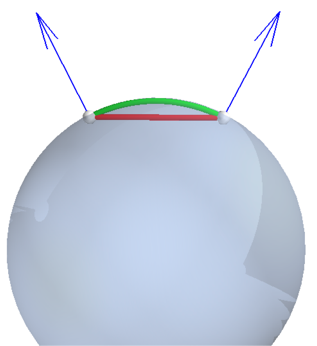
\includegraphics[width=0.9\textwidth]{statistical_normals/images/normal_distance}
		\captionof{figure}{The two arrow-headed vectors represents normals
		                   embedded on the surface of the unit sphere. The red
		                   line is the Euclidean distance, which underestimates
		                   the true distance. The green arc is the metrically
		                   correct geodesic distance.}
\label{fig:singl_img_norm_normal_distance}
	\end{minipage}
	\hspace{1cm}
	\begin{minipage}[t]{.45\textwidth}
		\centering
		
\includegraphics[width=0.9\textwidth]{statistical_normals/images/united_nations_logo}
		\captionof{figure}{The flag of the United Nations (UN) depicts
		                   an Azimuthal Equidistant projection centred on the
		                   North pole. Image of the UN flag is used under the
		                   terms of the public domain~\cite{un_flag}.}
\label{fig:singl_img_united_nations}
	\end{minipage}
\end{figure}
%%%%%%%%%%%%%%%%%%%%%%%%%%%%%%%%%%%%%%%%
Thus, any component analysis method that is to be performed on directional data
must be able to account for both non-Euclidean distance computation 
and the manifold constraints on the data mean. 
One method of computing component analysis on data that is
not related linearly and thus where Euclidean distances do not hold is
Kernel Principal Component Analysis (KPCA)~\cite{scholkopf1998nonlinear}.
KPCA is a non-linear generalisation of PCA that allows the computation
of component analysis within arbitrary dimensional Hilbert spaces,
including the subspace of normals. A Hilbert space is a generalisation
of a Euclidean space to arbitrary dimensions. More specifically, a Hilbert
space is a vector space possessing the structure of an inner
product. Thus, by providing a kernel function that defines
an inner product within a Hilbert space, we can perform component analysis in
spaces where PCA would normally be incorrect.

In this \namecref{ch:singl_imag}, we show the power of using KPCA to perform
component analysis of normals. The difference between the proposed framework and
previous works is that, instead of using off-the-shelf kernels such as Radial
Basis Functions (RBFs) or polynomial kernels, we are interested only in kernels
tailored to directional data. By incorporating the constraints of directional
data directly into our analysis we derive two novel kernels for performing
statistical analysis directly on normals. It is important to note that this is
not the first work to consider the construction of statistical models of surface
normals. \citet{smith2006recovering,smith2008facial} were the
first to note the complexities of performing component analysis on normals. To
solve this problem, \citet{smith2006recovering,smith2008facial}
proposed to borrow from the cartographic
community in order to define projection operators that map points on the surface
of a sphere to a tangent plane that preserves distances. This projection, called
the Azimuthal Equidistant Projection (AEP)~\cite{snyder1987map} is demonstrated
most commonly by the flag of the United Nations as depicted in
\cref{fig:singl_img_united_nations}.
\citet{smith2008facial} also investigated the use of
Principal Geodesic Analysis (PGA)~\cite{fletcher2004principal,smith2008facial}
for building statistical models of normals. In particular, PGA provides a
principled way to correctly compute the mean of a Riemannian manifold.
A Riemannian manifold is a differentiable manifold that is locally similar
enough to a linear space to allow for calculus. Specifically, a Riemannian
manifold defines an inner product on the tangent space such that distances
in the tangent space are preserved locally on the manifold. 

However,
although the observation that computing distances between normals is non-trivial
is correct, this does not actually prevent component analysis being computed
directly on normals (\ie~without applying any transformation). By formulating
the component analysis in terms of a kernel, it becomes obvious that component
analysis \textit{can be performed directly on normals by defining the kernel as
the Euclidean inner product or cosine kernel}. We generalise AEP and PGA as
kernels in our framework and provide novel kernels that allow for the
computation of component analysis directly on normals, without the need for
projection into a tangent space.

Another intriguing property of surface normals is that they encode a local
measurement of surface orientation. Naturally, this means that a field of
surface normals provide insight into the curvature of the surface. This encoding
of local curvature shares many similarities to the concept of gradients in the
image domain. In fact, as discussed in \cref{sec:bg_sfs}, surface normals may be
parametrised as a gradient field directly and assuming the gradient field to be
integrable, may be integrated to recover 3D shape. The parametrisation of
surface normals as gradient fields is particularly interesting given the work of
\citet{tzimiropoulos2012subspace,tzimiropoulos2011robust,%
tzimiropoulos2014active} who show that gradient orientations can be coupled with
the cosine function in order to perform robust comparisons between images. In
particular, \citet{tzimiropoulos2012subspace} show that using the
cosine of normalised gradients as a dissimilarity measure allows gradients
to be effectively used for both component
analysis~\cite{tzimiropoulos2012subspace,tzimiropoulos2014active} and alignment
purposes~\cite{tzimiropoulos2011robust,tzimiropoulos2014active,%
antonakos2015feature}. The main result of the work on the cosine of normalised
gradients is that gross outliers, such as occlusions, are effectively suppressed
by the cosine function assuming the outliers are drawn from particular
distributions. This is an important result as it implies that the effect
of gross outliers for dissimilarity measurement is greatly reduced
under the distribution of normalised image gradients combined with
the cosine function. Inspired by this, we also investigate how the cosine
function might be used in conjunction with surface normals in order to build
robust dissimilarity measures. Therefore, in a similar manner to
\citet{tzimiropoulos2012subspace,tzimiropoulos2011robust,tzimiropoulos2014active},
we investigate the distribution of surface normals when combined with the
cosine function and provide applications for both component analysis and
alignment. As mentioned, we show the application of Kernel PCA for surface
normals and provide two novel kernels which follow from the combination
of surface normals with the cosine function. We also investigate parametric
alignment within the Lucas-Kanade~\cite{lucas1981iterative} framework
by employing both the cosine dissimilarity directly and with a statistical
model of surface normals. Following recent works on robust feature spaces for
alignment~\cite{antonakos2015feature}
we show that performing well known alignment algorithms such as
Lucas-Kanade~\cite{lucas1981iterative} on image descriptors (or features) can
provide significant improvements in alignment. Given a statistical model
of normals, we further investigate the properties of normals for rigid and
deformable alignment within the Lucas-Kanade framework. Specifically, we
investigate two separate modalities of data, \textbf{2.5D data} as is
commonly supplied by depth cameras and \textbf{volumetric 3D data} as is more common
in the medical imaging community. For 2.5D data, we propose to use normals both
as a feature for Lucas-Kanade~\cite{lucas1981iterative} fitting,
as in the work of \citet{antonakos2015feature}, and as a statistical
appearance model for Active Appearance Model~\cite{cootes2001active} alignment.
For 3D data (or volumetric data), we provide two novel
inverse compositional alignment~\cite{baker2004lucas} algorithms for robustly
aligning data that contains gross outliers such as occlusions.

The rest of this chapter continues as follows:
\cref{sec:singl_img_cosine_orientations} describes the various
parameterisations of surface normals and discusses how they may be combined with
the cosine function. Preliminary examples are provided for multiple
data sources that experimentally verify that the cosine of surface normals
can provide a dissimilarity that is robust to gross outliers. Furthermore,
the use of surface normals for component analysis is discussed by proposing a
Kernel PCA framework for normals. It also embeds the existing AEP and PGA
operators as kernels.
\cref{sec:singl_img_gsfs} demonstrates how the KPCA framework augments
the geometric SfS method of \citet{worthington1999new} in a similar manner to
\citet{smith2006recovering}.
\cref{sec:singl_imag_lk} demonstrates how surface
normals can be utilised for alignment within Lucas-Kanade style
algorithms~\cite{lucas1981iterative}.
\cref{subsec:singl_img_lk_2d} demonstrates how a statistical model of normals
can be utilised to align 2.5D depth data by building an appearance model of
surface normals for use in an Active Appearance Model~\cite{cootes2001active}.
Finally, \cref{subsec:singl_img_lk_3d} demonstrates the use of normals for the
formation of a statistically robust rigid Lucas-Kanade~\cite{lucas1981iterative}
alignment method for 3D (volumetric) data.
%%%%%%%%%%%%%%%%%%%%%%%%%%%%%%%%%%%%%%%%%%%%%%%%%%%%%%%%%%%%%%%%%%%%%%%%%%%%%%%%
{
% List of mathematical commands for this chapter
\newcommand{\aepname}{\operatorname{AEP}}
\newcommand{\ipname}{\operatorname{IP}}
\newcommand{\sphername}{\operatorname{SPHER}}
\newcommand{\pganame}{\operatorname{PGA}}
\newcommand{\lsname}{\operatorname{LS}}

% Commands for KPCA
% Inner product mapping
\newcommand{\ip}{\Phi_{\ipname} (\bb{x}_k)}
% Inverse inner product mapping
\newcommand{\invip}{{\Phi_{\ipname}}^{-1} (\bb{v}_k)}
% Spherical mapping
\newcommand{\spher}{\Phi_{\sphername} (\bb{x}_k)}
% Inverse Spherical mapping
\newcommand{\invspher}{{\Phi_{\sphername}}^{-1} (\bb{v}_k)}
% AEP mapping
\newcommand{\aep}{\Phi_{\aepname} (\bb{x}_k)}
% Inverse AEP mapping
\newcommand{\invaep}{{\Phi_{\aepname}}^{-1} (\bb{v}_k)}
% PGA mapping
\newcommand{\pga}{\Phi_{\pganame} (\bb{x}_k)}
% Inverse PGA mapping
\newcommand{\invpga}{{\Phi_{\pganame}}^{-1} (\bb{v}_k)}
% Least squares mapping
\newcommand{\ls}{\Phi_{\lsname} (\bb{x}_k)}
% Inverse least squares mapping
\newcommand{\invls}{{\Phi_{\lsname}}^{-1} (\bb{v}_k)}


% Commands for Appendix
\newcommand{\g}{\bb{g}}
\newcommand{\tildeg}{\bb{\tilde{g}}}
\newcommand{\W}{\bb{W}}
\newcommand{\deltap}{\bb{\Delta{} p}}
\newcommand{\x}{\bb{x}}
\newcommand{\I}{\bb{I}}
\newcommand{\GTwo}{\bb{G_2}}
\newcommand{\GOne}{\bb{G_1}}
\newcommand{\J}{\bb{J}}
\newcommand{\zero}{\bb{0}}
\newcommand{\p}{\bb{p}}

%%%%%%%%%%%%%%%%%%%%%%%%%%%%%%%%%%%%%%%%%%%%%%%%%%%%%%%%%%%%%%%%%%%%%%%%%%%%%%%%
%%%%%%%%%%%%%%%%%%%%%%%%%%%%%%%%%%%%%%%%%%%%%%%%%%%%%%%%%%%%%%%%%%%%%%%%%%%%%%%%
\section{Cosine of Surface Orientations}\label{sec:singl_img_cosine_orientations}
%%%%%%%%%%%%%%%%%%%%%%%%%%%%%%%%%%%%%%%%%%%%%%%%%%%%%%%%%%%%%%%%%%%%%%%%%%%%%%%%
In this section we describe the theory behind building robust dissimilarity
measures by utilising the cosine function. In this work, we consider a
dissimilarity measure to be robust if it suppresses the contribution of
comparisons between image areas that are unrelated. More specifically, we seek a
measure that, when given two images that are visually dissimilar, will calculate
zero correlation between them. Suppressing the contribution of outliers is
a well studied area of mathematics and one flexible method of achieving this
is to employ a weighted comparison. A weighted comparison can be constructed
such that image areas that contain outliers are given a zero weighting and thus
do not bias the effect of comparing two images in regions excluding the outlier.
This is useful for applications such as facial image alignment whereby an image
may contain gross outliers in the form of occlusions such as ``hand over the
face'' gestures. In this scenario it is still appropriate to attempt to
align a facial model to the occluded input image and seek to suppress
the effect of the region of the face where the hand appears. This is also
appropriate in the case of statistical SfS which may also contain outliers
such as shadows and gesture occlusions. Unfortunately, identifying the outlier
regions is a challenging problem that likely requires complex scene
understanding in order to achieve accurately.
To this end, \citet{tzimiropoulos2012subspace} proposed the use of the cosine
function to provide a non-parametric method for suppressing outliers which
is shown to be equivalent to an automatically weighted dissimilarity measure.
Given the periodic domain of the cosine function is it desirable for the
input to also be bounded in a similar periodic range. For this reason,
\citet{tzimiropoulos2012subspace} propose to use polar coordinates to encode
the orientation of the normalised gradient, which is naturally bounded in the
$[0, 2\pi)$ range. This was utilized for both facial
alignment~\cite{tzimiropoulos2011robust,tzimiropoulos2014active,%
antonakos2015feature} and component
analysis~\cite{tzimiropoulos2012subspace,tzimiropoulos2014active}.

We propose to utilise the cosine function to construct robust dissimilarity
measures for surface normals. Given that surface normals also encode a local
measure of surface orientation they are well suited as inputs to the cosine
function. It is necessary, however, to make a clean distinction as to the
dimensionality of the data being considered. For the original work
on the cosine of normalised image gradients~\cite{tzimiropoulos2012subspace}
the input data were 2D images. In this work, we consider two forms of three
dimensional data: \textbf{2.5D data} and \textbf{3D or volumetric data}.
2.5D data is commonly represented in the form of surfaces and we define
the surface normal to be the unit vector perpendicular to the plane
tangent to a point on the surface. This surface normal contains
two degrees of freedom and is assumed to be a unit vector. 3D or volumetric
data is the direct extension of 2D images into the true third dimension
whereby the discrete elements composing the image are 3D voxels as opposed to
2D pixel. In this case, a true third dimension exists and gradients (which
are analogous to normals) are defined in a manner similar to 2D gradients. This
form of data is very common in the medical imaging community, for example.

The remainder of this section will explain the assumptions and theory around
utilising the cosine function as a robust dissimilarity measure. We then
provide uses of the measure in the form of parametric SfS, 2D face
alignment using depth data and volumetric image alignment.
%%%%%%%%%%%%%%%%%%%%%%%%%%%%%%%%%%%%%%%%%%%%%%%%%%%%%%%%%%%%%%%%%%%%%%%%%%%%%%%%
\subsection{Cosine Similarity in 2D}\label{subsec:cosine_2d}
%%%%%%%%%%%%%%%%%%%%%%%%%%%%%%%%%%%%%%%%%%%%%%%%%%%%%%%%%%%%%%%%%%%%%%%%%%%%%%%%
%TODO: Fix figures
%%%%%%%%%%%%%%%%%%%%%%%%%%%%%%%%%%%%%%%%
% \begin{figure*}
%     \centering
%     \hspace*{\fill}
%     \begin{subfigure}[t]{0.33\textwidth}
%         \centering
%         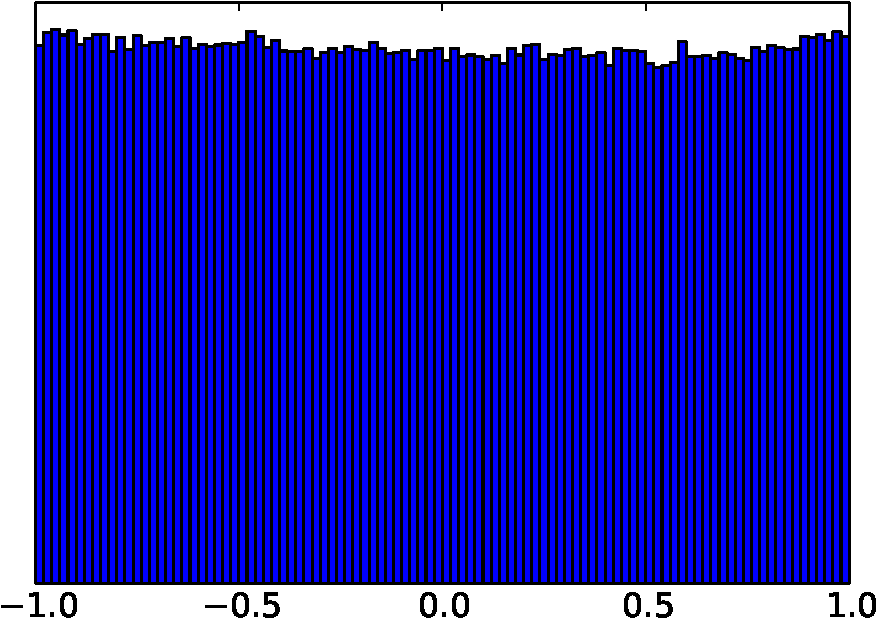
\includegraphics[width=\textwidth]{images/distributions/inner_product_tumour-crop}
%         \caption{$\cos{\sigma}$ tumour area}\label{subfig:inner_product_tumour}
%     \end{subfigure} \hfill
%     \begin{subfigure}[t]{0.32\textwidth}
%         \centering
%         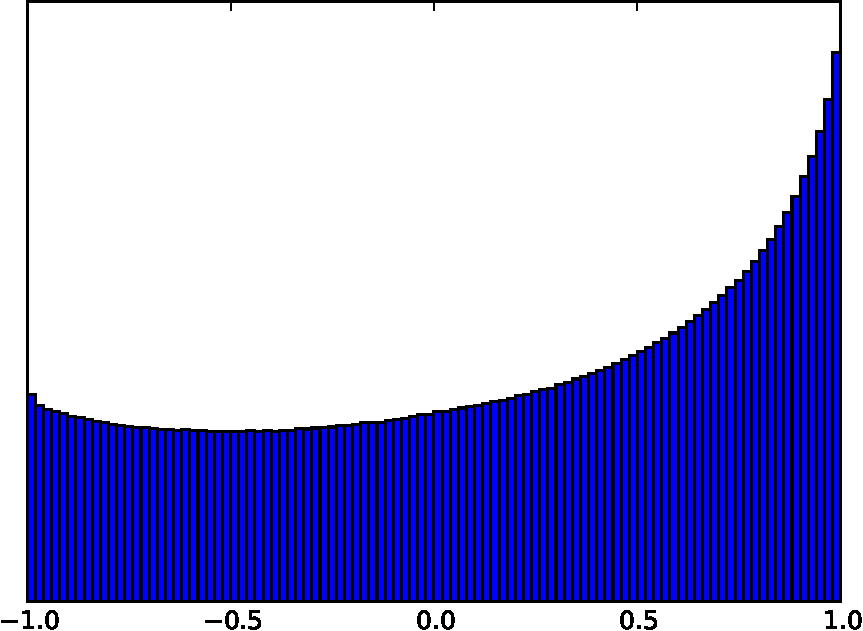
\includegraphics[width=\textwidth]{images/distributions/inner_product_all-crop}
%         \caption{$\cos{\sigma}$ entire image}\label{subfig:inner_product_all}
%     \end{subfigure} \hfill
%     \begin{subfigure}[t]{0.33\textwidth}
%         \centering
%         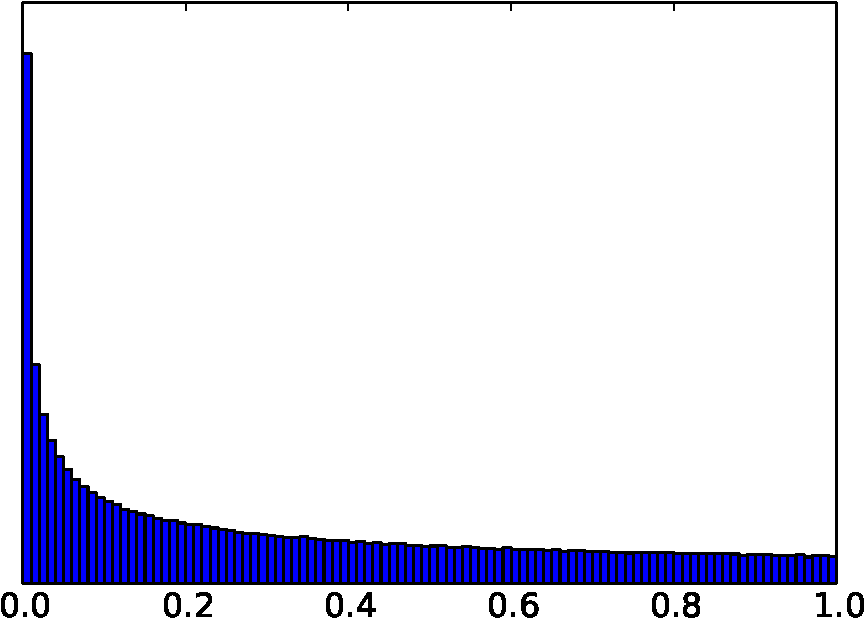
\includegraphics[width=\textwidth]{images/distributions/inner_product_squared_tumour-crop}
%         \caption{$\cos^{2}{\sigma}$ tumour area}\label{subfig:inner_product_squared_tumour}
%     \end{subfigure}
%     \hspace*{\fill}
%     \caption{The distributions of $\cos{\sigma}$ and $\cos^2{\sigma}$ averaged
%              over 10 subjects from the BraTS simulated images. The images were
%              registered using a rigid transformation prior to computation and
%              only the tumour areas were sampled. (a) shows the distribution of
%              $\cos{\sigma}$ in the simulated tumour region. (b) shows the
%              distribution of $\cos{\sigma}$ over the entire image. (c) shows the
%              distribution of $\cos^2{\sigma}$ proposed
%              in~\cite{haber2006intensity} in the simulated tumour region}
% \label{fig:inner_product_distributions}
% \end{figure*}
%%%%%%%%%%%%%%%%%%%%%%%%%%%%%%%%%%%%%%%%
Assuming we are given two 2D images, denoted as $I_i, \; i \in \{1,2\}$, we
define $G_{i,x} = \bb{F}_x \ast I_i$ and $G_{i,y} = \bb{F}_y \ast I_i$
as the gradients obtained by convolving $I_i$ with differentiation approximation
filters $\bb{F}_x$ and $\bb{F}_y$ respectively. We denote the
lexicographical vectorisation of $G_{i,x}$ as $\bb{g}_{i,x}$ and define an
index $k$ into the vector, $\bb{g}_{i,x}(k)$. We define an identical vector
for $G_{i,y}$ as $\bb{g}_{i,y}$. We also define $\bb{g}_{i}(k)$ as the
vector formed by concatenating the $x$ and $y$ gradients together. Trivially, we
can define the normalised gradient as
$\bb{\tilde{g}}_{i}(k) = \frac{\bb{g}_{i}(k)}{\norm{\bb{g}_{i}(k)}}$ where
$\norm{\bb{g}_{i}(k)} = \sqrt{{g_{i,x}(k)}^2 + {g_{i,y}(k)}^2}$.  We also define
similar vectors for the $x$ and $y$ components separately, with
$\bb{\tilde{g}}_{i,x}$ being the $x$ components concatenated in
lexicographical ordering and $\bb{\tilde{g}}_{i,y}$ being the $y$ components.
Finally, $\bb{\tilde{g}}_{i}$ is the vector of concatenated normalised
gradients for image $I_i$.

Given the normalised gradients, it is simple to parametrise them within a polar
coordinate system with radius $r_i(k) = \lVert \bb{\tilde{g}}_{i}(k) \rVert = 1$,
orientation $\phi_i(k) = \arctan{\frac{\tilde{g}_{i,y}(k)}{\tilde{g}_{i,x}(k)}}$
and pole at the origin.
Given orientations from two dissimilar images, it is reasonable to assume that
difference between the orientations, $\Delta \phi(k) = \phi_1(k) - \phi_2(k)$,
can take any angle between $[0, 2\pi)$. Intuitively, this implies that selecting
two pixels from dissimilar images is unlikely to yield any correlation between
the images. In~\cite{tzimiropoulos2011robust}, it was experimentally verified that the
orientation differences follow a uniform distribution, $\Delta \phi(k) \sim U(0,
2\pi)$. The fact that the orientation differences follows a uniform distribution
is unsurprising under the assumption that the two images have absolutely no
correlation. However, the expectation of the cosine of the uniform distribution
is zero, which is a powerful property that can be exploited for image
registration. It is powerful because it means that the expected overall
contribution of uncorrelated areas to any cost function will be zero, meaning
the uncorrelated areas do not affect the result of the registration.

Formally, we assume $\Delta \phi(k)$ is a stationary random process $y(t)$ with
index $t \triangleq k \in \mathcal{R}^2$, where $\forall t \sim U(0, 2\pi)$. We
define the random process $z(t) = \cos{y(t)}$ and thus $\forall t$ random
variable $Z = z(t)$ has mean value $E\{Z\} = 0$. In fact, by assuming mean
ergodicity, we find that
%%%%%%%%%%%%%%%%%%%%%%%%%%%%%%%%%%%%%%%%%%%%%%%%%%%%%%%%%%%%%%%%%%%%%%%%%
\begin{equation}\label{eq:cosine_integral}
    E\{Z\} \propto \int z(t) dt \equiv \int_{\mathcal{R}^2} \cos[\Delta \phi(k)] dk = 0
\end{equation}
%%%%%%%%%%%%%%%%%%%%%%%%%%%%%%%%%%%%%%%%%%%%%%%%%%%%%%%%%%%%%%%%%%%%%%%%%
This is an important property for a similarity measure to be robust against
occlusions. Since occlusions do not provide useful information for alignment,
ideally they would be ignored. However, manual segmentation of occluded areas is
time consuming and prone to error. Therefore, an ideal robust similarity measure
would be able to automatically identify regions of the image that are occluding
the true object of interest. Under the previous definition of robustness, the
cosine similarity naturally represents a robust similarity measure as it
automatically suppresses the contribution of outliers.

Given an image warping function with parameters $\bb{p}$, maximising the sum
of the cosine of orientation differences provides the robust similarity measure:
%%%%%%%%%%%%%%%%%%%%%%%%%%%%%%%%%%%%%%%%%%%%%%%%%%%%%%%%%%%%%%%%%%%%%%%%%
\begin{equation}\label{eq:2d_similarity_measure}
    q = \sum_k \cos \left(\Delta \phi(k)[\bb{p}]\right)
\end{equation}
%%%%%%%%%%%%%%%%%%%%%%%%%%%%%%%%%%%%%%%%%%%%%%%%%%%%%%%%%%%%%%%%%%%%%%%%%
For more details of the specifics of optimising (\ref{eq:2d_similarity_measure})
for image alignment, we refer the reader to~\cite{tzimiropoulos2011robust}.
%%%%%%%%%%%%%%%%%%%%%%%%%%%%%%%%%%%%%%%%%%%%%%%%%%%%%%%%%%%%%%%%%%%%%%%%%%%%%%%%
\subsection{Cosine Similarity in 3D}\label{subsec:cosine_3d}
%%%%%%%%%%%%%%%%%%%%%%%%%%%%%%%%%%%%%%%%%%%%%%%%%%%%%%%%%%%%%%%%%%%%%%%%%%%%%%%%
We make very similar assumptions for 3D images as we did in
\cref{subsec:cosine_2d} for 2D images. We simply extend the previous
notation by including the gradient of the $z$-axis, denoted as $G_{i,z} = \bb{F}_z \ast I_i$.
We also redefine the normalised gradient as
$\bb{\tilde{g}}_{i}(k) = \frac{\bb{g}_{i}(k)}{\norm{\bb{g}_{i}(k)}}$
where $\norm{\bb{g}_{i}(k)} = \sqrt{{g_{i,x}(k)}^2 + {g_{i,y}(k)}^2 +
{g_{i,z}(k)}^2}$ and $\bb{g}_{i}(k)$ is defined as the vector formed by
concatenating the $x$, $y$ and $z$ gradients together.

Measuring the angular distance between vectors in 3D is more complex than in 2D,
due to the extra degree of freedom. In the following sections, we describe two
different measures that can be used to calculate similarities between vectors
within 3D images, the spherical coordinates and the inner product. In the
previous section, we described in detail how properties of the cosine of a
uniform distribution can be exploited to form a robust measure of similarity.
The most important property was that uncorrelated areas such as occlusions
should have no impact registration. This was formalised as the expectation of
the sum of the uncorrelated elements should be zero. In the case of input to the
cosine function, a given distribution must simply be symmetric over the positive
and negative span of outputs of the cosine. When symmetric over the positive and
negative outputs, the expectation of the cosine function is zero. In fact, we
can relax the definition of a measure being robust to outliers by stating that
we desire a measure whereby the expectation of the measure over image areas that
are uncorrelated is zero.

In practise, when comparing two images where one image contains occlusions,
there will be regions that are correlated and then the occluded region that is
uncorrelated. In this case, the total distribution of all pixels will be
described by a mixture model of the occluded and non-occluded regions. We desire
that the distribution of the uncorrelated areas has an expectation of zero and
thus will not affect the optimisation of the similarity measure.

In \cref{subsubsec:cosine_spherical} and
\cref{subsubsec:cosine_inner_product} we describe two measures of angular
difference between 3D images. We investigate the distribution of these angular
measures when combined with the cosine function and motivate that they are both
suitable for use as a similarity measure between real 3D images.
%%%%%%%%%%%%%%%%%%%%%%%%%%%%%%%%%%%%%%%%%%%%%%%%%%%%%%%%%%%%%%%%%%%%%%%%%%%%%%%%
\subsubsection{Spherical Coordinates}\label{subsubsec:cosine_spherical}
%%%%%%%%%%%%%%%%%%%%%%%%%%%%%%%%%%%%%%%%%%%%%%%%%%%%%%%%%%%%%%%%%%%%%%%%%%%%%%%%
In 2D, a natural parametrisation of the angle between the two gradient vectors
is the polar coordinate system. In 3D, we have three gradient vectors and thus
require two angles to describe their orientation. Unlike in 2D, where the
vectors lie on the unit circle, in 3D the vectors lie on the surface of a unit
sphere. Therefore, it is possible to parametrise the vectors in terms of the
spherical coordinate system, which is described by two angles: the azimuth angle
$\phi$ with range $[0, 2\pi)$ and the elevation angle $\theta$ with range
$[0, \pi]$. Given the normalised gradients as vectors with Cartesian
coordinates, we can calculate the spherical angles as follows:
%%%%%%%%%%%%%%%%%%%%%%%%%%%%%%%%%%%%%%%%%%%%%%%%%%%%%%%%%%%%%%%%%%%%%%%%%
\begin{equation}\label{eq:cartesian_to_spherical}
    \begin{aligned}
        r_i(k)      &= \lVert \bb{\tilde{g}}_{i}(k) \rVert = 1            \\
        \phi_i(k)   &= \arctan{\frac{\tilde{g}_{i,y}(k)}{\tilde{g}_{i,x}(k)}} \\
        \theta_i(k) &= \arccos{\tilde{g}_{i,z}(k)}
    \end{aligned}
\end{equation}
%%%%%%%%%%%%%%%%%%%%%%%%%%%%%%%%%%%%%%%%%%%%%%%%%%%%%%%%%%%%%%%%%%%%%%%%%
An illustration of the spherical coordinate system, as used in this paper, is
given in \cref{fig:spherical_coordinates}.

Our proposal is to combine the spherical coordinates with the cosine function in
order to provide a robust similarity measure. Similar to the 2D case,, we
propose the cosine of azimuth differences, $\Delta \phi = \phi_1 - \phi_2$, and
the cosine of elevation differences, $\Delta \theta = \theta_1 - \theta_2$, as a
combined similarity measures. Given a 3D image warping function with parameters
$\bb{p}$, the spherical coordinates form a similarity measure as follows:
%%%%%%%%%%%%%%%%%%%%%%%%%%%%%%%%%%%%%%%%%%%%%%%%%%%%%%%%%%%%%%%%%%%%%%%%%
\begin{equation}\label{eq:spherical_similarity_measure}
    q = \sum_k \cos \left(\Delta \phi(k)[\bb{p}]\right) + \sum_k \cos \left(\Delta \theta(k)[\bb{p}]\right)
\end{equation}
%%%%%%%%%%%%%%%%%%%%%%%%%%%%%%%%%%%%%%%%%%%%%%%%%%%%%%%%%%%%%%%%%%%%%%%%%
Optimisation of (\ref{eq:2d_similarity_measure}) is described in detail in
\cref{sec:robust_lk}.

Experimentally, we verified that $\Delta \phi$ approximates a symmetric
distribution for simulated tumour data taken from the Multimodal Brain Tumor
Image Segmentation (BraTS) challenge, as shown in
\cref{fig:phi_distribution}. \cref{subfig:phi_tumour} shows the
distribution of $\Delta \phi$ between the tumour area circled in yellow in
\cref{fig:tumour_examples} and a healthy brain. The images were registered
using a rigid transformation before $\Delta \phi$ was computed.  The azimuth
angle is analogous to the angle studied in~\cite{RefWorks:68} and follows the
same uniform distribution, $\Delta \phi \sim U(0, 2\pi)$.

When the entire region of the rigidly registered brain images is considered, we
find that the distribution of $\Delta \phi$ is clearly a mixture of two separate
models, one for the occluded area and one for the rigidly registered area.
\cref{subfig:phi_all} shows the distribution of $\Delta \phi$ calculated
over the entire image region of each image and a Laplacian distribution that
best fits the data. Thus, our experimental evidence suggests that the total
distribution of $\Delta \phi$ over the entire image region is a mixture model
between a uniform distribution and a Laplacian distribution with approximately
zero mean.
% The elevation angle, however, appears to have a very interesting and novel distribution. \cref{fig:delta_theta} shows that the distribution of $\Delta \theta$ approximates a Von Mises distribution. Therefore, given the range of $\Delta \theta$, \cref{fig:sin_delta_theta} shows that the correct robust function for $\Delta \theta$ is in fact the sine function, $\sin{\Delta \theta}$. Although \cref{fig:sin_delta_theta} has heavy tails at $-1$ and $1$, the distribution is symmetric and has been experimentally verified to have an expected value of $0$. However, since $\Delta \theta$ is symmetric over the range of the sine function and since (\ref{eq:cosine_integral}) holds analogously for the sine function, then $\sin{\Delta \theta}$ represents a robust measure of similarity.
%%%%%%%%%%%%%%%%%%%%%%%%%%%%%%%%%%%%%%%%
% \begin{figure}
%     \centering
%     \begin{subfigure}{0.32\columnwidth}
%         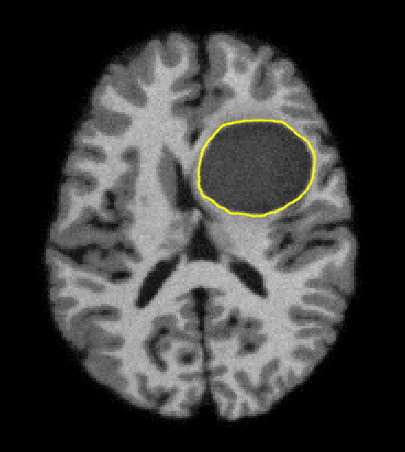
\includegraphics[width=\textwidth]{images/tumour_example_axial}
%     \end{subfigure}
%     \begin{subfigure}{0.32\columnwidth}
%         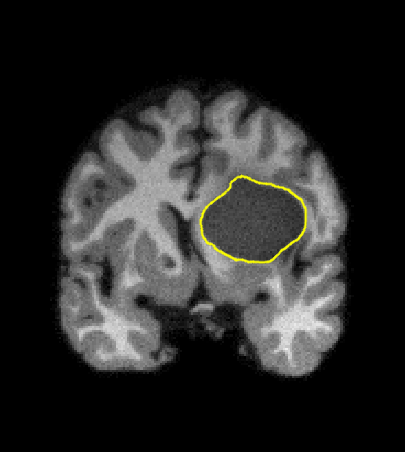
\includegraphics[width=\textwidth]{images/tumour_example_coronal}
%     \end{subfigure}
%     \begin{subfigure}{0.32\columnwidth}
%         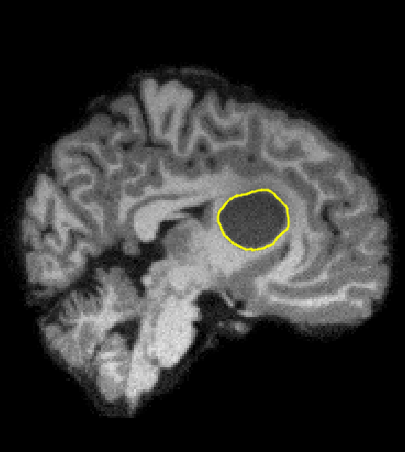
\includegraphics[width=\textwidth]{images/tumour_example_sagital}
%     \end{subfigure}
%     \caption{Example images of a T1-weighted brain containing a tumour area.
%              The tumour areas are outlined in yellow in each image.
%              Left: Axial View. Middle: Coronal View. Right: Sagital View.}
% \label{fig:tumour_examples}
% \end{figure}
%%%%%%%%%%%%%%%%%%%%%%%%%%%%%%%%%%%%%%%%
% %%%%%%%%%%%%%%%%%%%%%%%%%%%%%%%%%%%%%%%%
% \begin{figure}
%     \centering
%     \begin{subfigure}{0.47\columnwidth}
%         \includegraphics[width=\textwidth]{images/tumour_example_3d}
%     \end{subfigure}
%     \begin{subfigure}{0.47\columnwidth}
%         \includegraphics[width=\textwidth]{images/healthy_example_3d}
%     \end{subfigure}
%     \caption{Example images of T1-weighted brain images of a single individual.
%              Left: Simulated tumour.
%              Right: The original healthy brain.}
% \label{fig:3d_tumour_example}
% \end{figure}
% %%%%%%%%%%%%%%%%%%%%%%%%%%%%%%%%%%%%%%%%
%%%%%%%%%%%%%%%%%%%%%%%%%%%%%%%%%%%%%%%%%%%%%%%%%%%%%%%%%%%%%%%%%%%%%%%%%%%%%%%%
\subsubsection{Inner Product}\label{subsubsec:cosine_inner_product}
%%%%%%%%%%%%%%%%%%%%%%%%%%%%%%%%%%%%%%%%%%%%%%%%%%%%%%%%%%%%%%%%%%%%%%%%%%%%%%%%
A more general angular measure between two vectors is the inner product. Unlike
in~\cite{tzimiropoulos2011robust} or \cref{subsubsec:cosine_spherical}, the inner
product is a single angle and not the difference between two angles.
Practically, the inner product measures the projection error between two vectors
and is defined as:
%%%%%%%%%%%%%%%%%%%%%%%%%%%%%%%%%%%%%%%%%%%%%%%%%%%%%%%%%%%%%%%%%%%%%%%%%
\begin{equation}\label{eq:inner_product}
    \cos{\sigma} = \bb{\tilde{g}}_{1}^{\top} \bb{\tilde{g}}_{2}
\end{equation}
%%%%%%%%%%%%%%%%%%%%%%%%%%%%%%%%%%%%%%%%%%%%%%%%%%%%%%%%%%%%%%%%%%%%%%%%%
In~\cite{RefWorks:68}, the authors reasonably propose that the angle between the
gradients of dissimilar images can take any value in $[0, 2\pi)$ with equal
probability. Similarly, the relationship between the gradient vectors of two
dissimilar 3D images could feasibly be in any direction with equal probability.
Therefore, the distribution of inner products between two unrelated vectors can
take the values $[-1, 1]$ with equal probability. Due to the expected range of
inner product values, we would expect that $\cos{\sigma}$ follows a uniform
distribution, $\cos{\sigma} \sim U(-1, 1)$. Note that this is a different
assumption to that made in~\cite{RefWorks:68}, which assumes that the
\textit{azimuth angle itself}, $\Delta \phi$, follows a uniform distribution.
However, it is merely sufficient that the total sum of values from the
dissimilar vectors is zero. Therefore, since $E\{U(-1, 1)\} = 0$, the inner
product of normalised gradients satisfies our definition of being robust to
outliers. In \cref{subfig:inner_product_tumour}, we show that this
assumption holds for the simulated tumour data taken from the BraTS challenge.

When the entire region of the rigidly registered brain images is considered, we
find that the distribution of $\cos{\sigma}$ is clearly a mixture of two
separate models, one for the occluded area and one for the rigidly registered
area. \cref{subfig:inner_product_all} shows the distribution of
$\cos{\sigma}$ calculated over the entire image region. In this case, the
distribution of the inner product appears to be a mixture model between a
uniform distribution and a zero mean Laplacian distribution. However, due to the
ambiguity in the inner product in terms of orientation, the angle of the inner
product is only defined in the range $[0, \pi]$ and thus only the positive tail
of the Laplacian appears.

In \cref{subfig:inner_product_squared_tumour} we also show the
distribution of the similarity measure proposed by \citet{haber2006intensity}.
In~\cite{haber2006intensity}, the authors propose the inner product as a
similarity measure, which looks very similar to the measure we proposed in
\cref{eq:inner_product}. However, \citet{haber2006intensity} maximise the square of the
inner product using a least squares Gauss-Newton optimisation. As we have shown,
the inner product is related to the cosine between the vectors.
\citet{haber2006intensity} proposed the inner product squared as
a similarity, which is equivalent to the \textit{square of the cosine}. As we
can see in \cref{subfig:inner_product_squared_tumour}, the cosine squared
does not represent a symmetric distribution and therefore is not a robust
similarity measure by our definition.
%%%%%%%%%%%%%%%%%%%%%%%%%%%%%%%%%%%%%%%%
% \begin{figure}
%     \centering
%     \hspace*{\fill}
%     \begin{subfigure}[b]{0.46\columnwidth}
%     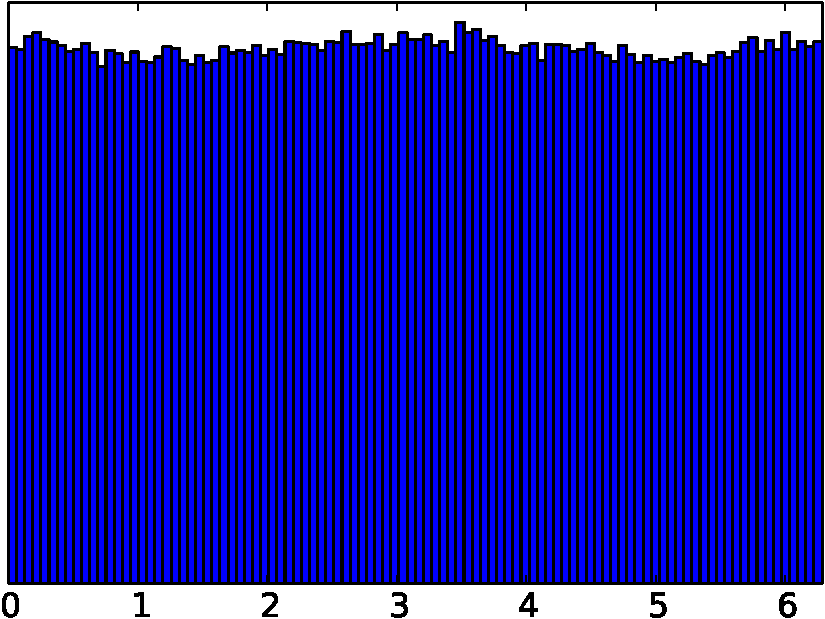
\includegraphics[width=\textwidth]{images/distributions/delta_phi_tumour-crop}
%     \caption{}\label{subfig:phi_tumour}
%     \end{subfigure}
%     \hfill
%     \begin{subfigure}[b]{0.45\columnwidth}
%     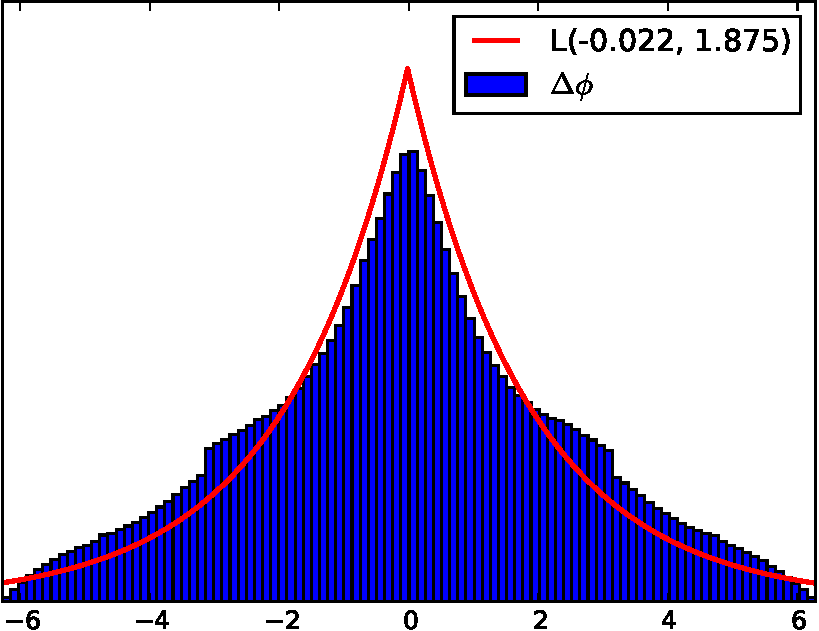
\includegraphics[width=\textwidth]{images/distributions/delta_phi_all_laplacian-crop}
%     \caption{}\label{subfig:phi_all}
%     \end{subfigure}
%     \hspace*{\fill}
%     \caption{The mean distribution of $\Delta \phi$ of the BraTS simulated images.
%              The images were registered using a
%              rigid transformation and only the tumour
%              areas were sampled. (a) the distribution of $\Delta \phi$
%              in the simulated tumour region. (b) the distribution of
%              $\Delta \phi$ over the entire image. It also shows the
%              Laplacian distribution that best fits the data.}
% \label{fig:phi_distribution}
% \end{figure}
%%%%%%%%%%%%%%%%%%%%%%%%%%%%%%%%%%%%%%%%
%%%%%%%%%%%%%%%%%%%%%%%%%%%%%%%%%%%%%%%%%%%%%%%%%%%%%%%%%%%%%%%%%%%%%%%%%%%%%%%%

%%%%%%%%%%%%%%%%%%%%%%%%%%%%%%%%%%%%%%%%%%%%%%%%%%%%%%%%%%%%%%%%%%%%%%%%%%%%%%%%
%%%%%%%%%%%%%%%%%%%%%%%%%%%%%%%%%%%%%%%%%%%%%%%%%%%%%%%%%%%%%%%%%%%%%%%%%%%%%%%%
\subsection{Component Analysis of Surface Normals}\label{subsec:singl_img_ca}
%%%%%%%%%%%%%%%%%%%%%%%%%%%%%%%%%%%%%%%%%%%%%%%%%%%%%%%%%%%%%%%%%%%%%%%%%%%%%%%%
%%%%%%%%%%%%%%%%%%%%%%%%%%%%%%%%%%%%%%%%%%%%%%%%%%%%%%%%%%%%%%%%%%%%%%%%%%%%%%%%
\subsubsection{Kernel PCA}\label{subsubsec:singl_img_ca_kpca}
%%%%%%%%%%%%%%%%%%%%%%%%%%%%%%%%%%%%%%%%%%%%%%%%%%%%%%%%%%%%%%%%%%%%%%%%%%%%%%%%
Given a set of, $K$, $F$-dimensional data vectors stacked in a
matrix $\mathbf{X} = [\mathbf{x}_1, \ldots, \mathbf{x}_K] \in \R^F$, 
we assume the existence of a positive semi-definite kernel function 
$k(\circ, \circ) : \R^F \times \R^F \rightarrow \R$. Given that $k(\circ, \circ)$ 
is positive semi-definite we can use it to define the inner product in an 
arbitrary dimensional Hilbert space, $\hilbert$, which we will call the feature 
space. There then exists an implicit mapping, $\Phi$, from the input 
space $\R^F$ to the feature space, $\hilbert$:
%%%%%%%%%%%%%%%%%%%%%%%%%%%%%%%%%%%%%%%%%%%%
\begin{equation}
    \begin{aligned}\label{eq:implicit-map}
        \Phi : \R^F \rightarrow \hilbert, \; \; \mathbf{x} \rightarrow \Phi(\mathbf{x})
    \end{aligned}
\end{equation}
%%%%%%%%%%%%%%%%%%%%%%%%%%%%%%%%%%%%%%%%%%%%
Due to the often implicit nature of the mapping $\Phi$, we need only the kernel 
function since 
$\langle \Phi(\mathbf{x}_i), \Phi(\mathbf{x}_j) \rangle  = k (\mathbf{x}_i, \mathbf{x}_j)$, 
the so-called kernel trick. Now, component analysis within the feature space 
is equivalent to
%%%%%%%%%%%%%%%%%%%%%%%%%%%%%%%%%%%%%%%%%%%%
\begin{equation}
    \begin{aligned}\label{eq:feature-space-pca}
        \underset{\mathbf{U}_\Phi}{\arg\max} \; \mathbf{U}_\Phi^T \bar{\mathbf{X}}_\Phi \bar{\mathbf{X}}_\Phi^T \mathbf{U}_\Phi \qquad \text{s.t.} \; \mathbf{U}_\Phi^T \mathbf{U}_\Phi = \mathbf{I}
    \end{aligned}
\end{equation}
%%%%%%%%%%%%%%%%%%%%%%%%%%%%%%%%%%%%%%%%%%%%
where $\mathbf{U}_\Phi = [\mathbf{U}_\Phi^1, ..., \mathbf{U}_\Phi^P] \in \hilbert$,
$\mathbf{m}_\Phi = \frac{1}{K} \sum \limits_{i=1}^K \Phi(\mathbf{x_i})$ and
$\bar{\mathbf{X}}_\Phi = [\Phi(\mathbf{x_i}) - \mathbf{m}_\Phi, ..., \Phi(\mathbf{x_K}) - \mathbf{m}_\Phi]$.

By noting that 
$\mathbf{\bar{X}}_\Phi \mathbf{\bar{X}}_\Phi^T = (\mathbf{X}_\Phi \mathbf{M}) (\mathbf{X}_\Phi \mathbf{M})^T$, 
where $\mathbf{M} = \mathbf{I} - \frac{1}{K} \mathbf{1} \mathbf{1}^T$ and
$\mathbf{1}$ represents a vector of ones, we can find
$\mathbf{U}_\Phi$ by performing eigenanalysis on
$\bar{\mathbf{X}}_\Phi^T \bar{\mathbf{X}}_\Phi$. Therefore,
%%%%%%%%%%%%%%%%%%%%%%%%%%%%%%%%%%%%%%%%%%%%
\begin{equation}
    \begin{aligned}\label{eq:x-bar-corr}
        \mathbf{\bar{X}}_\Phi^T \mathbf{\bar{X}}_\Phi = \mathbf{V} \boldsymbol{\Lambda} \mathbf{V}^T \mathbf{U}_{\Phi} &= \mathbf{\bar{X}}_\Phi^T \mathbf{V} \boldsymbol{\Lambda}^{-\frac{1}{2}}
    \end{aligned}
\end{equation}
%%%%%%%%%%%%%%%%%%%%%%%%%%%%%%%%%%%%%%%%%%%%
Though $\mathbf{U}_\Phi$ can be defined, it cannot be calculated explicitly. 
However, we can compute the KPCA-transformed feature vector
 $\mathbf{\tilde{y}} = [\mathbf{y}_1, ..., \mathbf{y}_K]$ by:
%%%%%%%%%%%%%%%%%%%%%%%%%%%%%%%%%%%%%%%%%%%%
\begin{equation}
    \begin{aligned}\label{eq:projections}
        \mathbf{\tilde{y}} = \mathbf{U}_\Phi^T \Phi(\mathbf{y}) &= \boldsymbol{\Lambda}^{-\frac{1}{2}} \mathbf{V}^T \mathbf{\bar{X}}_\Phi^T \Phi(\mathbf{y}) \\
        &= \boldsymbol{\Lambda}^{-\frac{1}{2}} \mathbf{V}^T \mathbf{M} \mathbf{X}_\Phi^T \Phi(\mathbf{y})
    \end{aligned}
\end{equation}
%%%%%%%%%%%%%%%%%%%%%%%%%%%%%%%%%%%%%%%%%%%%
We can, therefore, define the projection in terms of the kernel function
%%%%%%%%%%%%%%%%%%%%%%%%%%%%%%%%%%%%%%%%%%%%
\begin{equation}\label{eq:kernel-vector}
        \mathbf{X}_\Phi^T \Phi(\mathbf{y}) = \left[ k(\mathbf{y}_1, \mathbf{x}_1), \ldots, k(\mathbf{y}_K, \mathbf{x}_K) \right]^T
\end{equation}
%%%%%%%%%%%%%%%%%%%%%%%%%%%%%%%%%%%%%%%%%%%%
Reconstruction of a vector can be performed by
%%%%%%%%%%%%%%%%%%%%%%%%%%%%%%%%%%%%%%%%%%%%
\begin{equation}\label{eq:vector-reconstruction}
        \bb{\tilde{X}} = {\Phi}^{-1} \left( \mathbf{U}_{\Phi} {\mathbf{U}_{\Phi}}^T (\Phi(\mathbf{x}) - \mathbf{m}_{\Phi}) + \mathbf{m}_{\Phi} \right)
\end{equation}
%%%%%%%%%%%%%%%%%%%%%%%%%%%%%%%%%%%%%%%%%%%%
Unfortunately, since ${\Phi}^{-1}$ rarely exists or is extremely expensive to 
compute, performing reconstruction using \cref{eq:vector-reconstruction} is not 
generally feasible. In these cases, reconstruction can be performed by means of 
pre-images~\cite{kwok2004pre}. However, in the case of the kernels we propose
for normals, ${\Phi}^{-1}$ does exist and explicit mapping between the space of
normals and kernel space is performed. Finally, we should note here that in the 
general KPCA framework it is not necessary to subtract the mean. In this case, 
KPCA can be seen in the perspective of metric multi-dimensional 
scaling~\cite{williams2002connection}.
%%%%%%%%%%%%%%%%%%%%%%%%%%%%%%%%%%%%%%%%%%%%%%%%%%%%%%%%%%%%%%%%%%%%%%%%%%%%%%%%

%%%%%%%%%%%%%%%%%%%%%%%%%%%%%%%%%%%%%%%%%%%%%%%%%%%%%%%%%%%%%%%%%%%%%%%%%%%%%%%%
%%%%%%%%%%%%%%%%%%%%%%%%%%%%%%%%%%%%%%%%%%%%%%%%%%%%%%%%%%%%%%%%%%%%%%%%%%%%%%%%
\subsubsection{Inner Product Kernel}\label{subsubsec:sing_img_ip_kernel}
%%%%%%%%%%%%%%%%%%%%%%%%%%%%%%%%%%%%%%%%%%%%%%%%%%%%%%%%%%%%%%%%%%%%%%%%%%%%%%%%
Given that the Euclidean inner product is well defined for normals, as 
described in \cref{subsubsec:singl_img_cosine_inner_product}, 
we can define a kernel of the form
%%%%%%%%%%%%%%%%%%%%%%%%%%%%%%%%%%%%%%%%%%%%
\begin{equation}\label{eq:ip-cosine-kernel}
    k(\mathbf{x}_i, \mathbf{x}_j) = \sum^K_k {\mathbf{n}_k^i}^T \mathbf{n}_k^j = \sum^K_k \cos \alpha^{ij}_k
\end{equation}
%%%%%%%%%%%%%%%%%%%%%%%%%%%%%%%%%%%%%%%%%%%%
where $\alpha^{ij}_k = \langle \mathbf{n}^i_k, \mathbf{n}^j_k \rangle$.

Subtracting the mean would affect the calculation of the cosine and thus would 
not preserve the cosine distance. Therefore, we note that the inner product 
mapping is equivalent to performing PCA without subtracting the mean. We refer 
to this kernel as the inner product (IP) kernel, and denote it as:
%%%%%%%%%%%%%%%%%%%%%%%%%%%%%%%%%%%%%%%%%%%%
\begin{equation}\label{eq:ip-kernel}
    \ip = \mathbf{x}_k
\end{equation}
%%%%%%%%%%%%%%%%%%%%%%%%%%%%%%%%%%%%%%%%%%%%
We can explicitly define the inverse mapping for the inner product as the 
normalisation of each individual normal within the feature space vector,
 $\mathbf{v}_k$:
%%%%%%%%%%%%%%%%%%%%%%%%%%%%%%%%%%%%%%%%%%%%
\begin{equation}\label{eq:inv-ip-kernel}
    \invip = \left[ x_k^1, y_k^1, z_k^1, \ldots, x_k^N, y_k^N, z_k^N \right]^T
\end{equation}
%%%%%%%%%%%%%%%%%%%%%%%%%%%%%%%%%%%%%%%%%%%%

After computing $\ip$, we estimate $\mathbf{U}_{IP}$ from 
\cref{eq:feature-space-pca} and set $\mathbf{M} = \mathbf{I}$. 
Reconstruction of a test vector of normals $\mathbf{x}$ is performed via
%%%%%%%%%%%%%%%%%%%%%%%%%%%%%%%%%%%%%%%%%%%%
\begin{equation}\label{eq:ip-reconstruction}
   \tilde{\mathbf{x}} = {\Phi_{IP}}^{-1} \left( \mathbf{U}_{IP} {\mathbf{U}_{IP}}^T \Phi_{IP}(\mathbf{x}) \right)
\end{equation}
%%%%%%%%%%%%%%%%%%%%%%%%%%%%%%%%%%%%%%%%%%%%
%%%%%%%%%%%%%%%%%%%%%%%%%%%%%%%%%%%%%%%%%%%%%%%%%%%%%%%%%%%%%%%%%%%%%%%%%%%%%%%%
\subsubsection{AEP Kernel}\label{subsubsec:sing_img_aep_kernel}
%%%%%%%%%%%%%%%%%%%%%%%%%%%%%%%%%%%%%%%%%%%%%%%%%%%%%%%%%%%%%%%%%%%%%%%%%%%%%%%%
The azimuthal equidistant projection (AEP)~\cite{snyder1987map,smith2006recovering} is a
cartographic projection often used for creating charts centred on the north
pole. The projection has the useful property that all lines that pass through
the centre of the projection represent geodesics on the surface of a sphere. The
projection is constructed at a point $P$ on the surface of a sphere by
projecting a local neighbourhood of points around $P$ onto the tangent plane
defined at $P$. In terms of normals, we construct the projection by calculating
the average normal across the training set at each point, and then projecting
each normal on to this tangent plane. This means that the local coordinate
system at each point is mean-centred according to the total distribution.

The AEP takes each normal, $\mathbf{n}_k^i$ and maps it to a new location on
a tangent plane, $\mathbf{v}_k^i = [\bar{x}_k^i, \bar{y}_k^i]^T$. The
inverse AEP takes the points  $v_k^i$ on the tangent plane and maps them back to
normals. For a more detailed derivation of the Azimuthal Equidistant Projection,
we invite the reader to consult the work of \citet{smith2006recovering}. Assuming each
normal has been projected to its tangent plane according to the AEP function, we
define the AEP mapping function as
%%%%%%%%%%%%%%%%%%%%%%%%%%%%%%%%%%%%%%%%%%%%
\begin{equation}\label{eq:aep-kernel}
    \aep = \left[ \bar{x}_k^1, \bar{y}_k^1, \ldots, \bar{x}_k^N, \bar{y}_k^N \right]^T
\end{equation}
%%%%%%%%%%%%%%%%%%%%%%%%%%%%%%%%%%%%%%%%%%%%
and also explicitly define the inverse mapping function
%%%%%%%%%%%%%%%%%%%%%%%%%%%%%%%%%%%%%%%%%%%%
\begin{equation}\label{eq:inv-aep-kernel}
    \invaep = \left[ x_k^1, y_k^1, z_k^1, \dots, x_k^N, y_k^N, z_k^N \right]^T
\end{equation}
%%%%%%%%%%%%%%%%%%%%%%%%%%%%%%%%%%%%%%%%%%%%
After computing $\aep$, we estimate $\mathbf{U}_{AEP}$ from 
\cref{eq:feature-space-pca} and set $\mathbf{M} = \mathbf{I}$. Reconstruction 
of a test vector of normals $\mathbf{x}$ is performed via
%%%%%%%%%%%%%%%%%%%%%%%%%%%%%%%%%%%%%%%%%%%%
\begin{equation}\label{eq:aep-reconstruction}
   \tilde{\mathbf{x}} = {\Phi_{AEP}}^{-1} \left( \mathbf{U}_{AEP} {\mathbf{U}_{AEP}}^T \Phi_{AEP}(\mathbf{x}) \right)
\end{equation}
%%%%%%%%%%%%%%%%%%%%%%%%%%%%%%%%%%%%%%%%%%%%
In~\cite{smith2006recovering}, $\mathbf{U}_{AEP}$ has been used as a prior to
perform facial shape-from-shading.
%%%%%%%%%%%%%%%%%%%%%%%%%%%%%%%%%%%%%%%%%%%%%%%%%%%%%%%%%%%%%%%%%%%%%%%%%%%%%%%%
\subsubsection{PGA Kernel}\label{subsubsec:singl_img_pga_kernel}
%%%%%%%%%%%%%%%%%%%%%%%%%%%%%%%%%%%%%%%%%%%%%%%%%%%%%%%%%%%%%%%%%%%%%%%%%%%%%%%%
Principal geodesic analysis (PGA)~\cite{fletcher2004principal,smith2008facial} replaces the
linear subspace normally created by PCA by a geodesic manifold. PGA can be used
to represent geodesic distances on the surface on any manifold, however, we
focus on its use on 2-spheres. This means that every principal component in PGA
on 2-spheres represents a great circle. The \textit{extrinsic mean}, as
described by \citet{pennec2006intrinsic}, calculated for PCA does not represent
an accurate distance on the manifold. Therefore, we choose to use the
\textit{intrinsic mean} defined by the Riemannian distance between two points,
$d(\circ,\circ)$. Assuming a set of data points $\mathbf{x}$ on embedded on
a 2-sphere, $S^2$, we can define the intrinsic mean as $\mu =
{\arg\min}_{\mathbf{x} \in S^2} \sum_i^K d(\mathbf{x},
\mathbf{x}_i)$.

Two important operators for the 2-sphere manifold are the logarithmic and
exponential maps. Given a point on the surface of a sphere and the normal
$\mathbf{n}$ at that point, we can define a plane tangent to the sphere at
$\mathbf{n}$. If we then have a vector $\mathbf{v}$, that points to
another point on the tangent plane, we can define the exponential map,
$Exp_{\mathbf{n}}$, as the point on the sphere that is distance
$\norm{\mathbf{v}}$ along the geodesic in the direction of $\mathbf{v}$
from $\mathbf{n}$. The logarithmic map, $Log_{\mathbf{n}}$ is the
inverse of the exponential map. Given a point on the surface of the sphere it
returns the corresponding point on the tangent plane at $n$. Given the
definition of the logarithmic map, we can define the Riemannian distance for a
2-sphere as $d(\mathbf{n}, \mathbf{v}) = \norm{Log_{\mathbf{n}}(\mathbf{v})}$.

However, as shown by \citet{smith2008facial}, PGA amounts to
performing PCA on the vectors $Log_\mu(\mathbf{n}_k)$. Therefore, a kernel-
based version of PGA has a mapping function equal to the logarithmic map and an
inverse mapping function equal to the exponential map. Assuming we have pre-
calculated the intrinsic means, $\mu^i$, we can explicitly define the PGA
mapping function as
%%%%%%%%%%%%%%%%%%%%%%%%%%%%%%%%%%%%%%%%%%%%
\begin{equation}\label{eq:pga-kernel}
    \pga = \left[ Log_{\mu^1}(\mathbf{n}_k^1), \ldots, Log_{\mu^N}(\mathbf{n}_k^N) \right]^T
\end{equation}
%%%%%%%%%%%%%%%%%%%%%%%%%%%%%%%%%%%%%%%%%%%%
and the inverse mapping as 
%%%%%%%%%%%%%%%%%%%%%%%%%%%%%%%%%%%%%%%%%%%%
\begin{equation}\label{eq:inv-pga-kernel}
    \invpga = \left[ Exp_{\mu^1}(\mathbf{v}_k^1), \ldots, Exp_{\mu^N}(\mathbf{v}_k^N) \right]^T
\end{equation}
%%%%%%%%%%%%%%%%%%%%%%%%%%%%%%%%%%%%%%%%%%%%
After computing $\pga$, we estimate $\mathbf{U}_{PGA}$ from 
\cref{eq:feature-space-pca} and set $\mathbf{M} = \mathbf{I}$. Reconstruction 
of a test vector of normals $\mathbf{x}$ is performed via
%%%%%%%%%%%%%%%%%%%%%%%%%%%%%%%%%%%%%%%%%%%%
\begin{equation}\label{eq:pga-reconstruction}
   \tilde{\mathbf{x}} = {\Phi_{PGA}}^{-1} \left( \mathbf{U}_{PGA} {\mathbf{U}_{PGA}}^T \Phi_{PGA}(\mathbf{x}) \right)
\end{equation}
%%%%%%%%%%%%%%%%%%%%%%%%%%%%%%%%%%%%%%%%%%%%
In~\cite{smith2008facial}, $\mathbf{U}_{PGA}$ has been used as a prior to
perform facial shape-from-shading.
%%%%%%%%%%%%%%%%%%%%%%%%%%%%%%%%%%%%%%%%%%%%%%%%%%%%%%%%%%%%%%%%%%%%%%%%%%%%%%%%
\subsubsection{Spherical Cosine Kernel}\label{subsubsec:singl_img_cosine_kernel}
%%%%%%%%%%%%%%%%%%%%%%%%%%%%%%%%%%%%%%%%%%%%%%%%%%%%%%%%%%%%%%%%%%%%%%%%%%%%%%%%
As described in \cref{subsubsec:singl_img_cosine_spherical}, the distance between
two normals can also be expressed in terms of spherical coordinates. Motivated
by the recent findings on the robustness of the cosine 
kernel~\cite{tzimiropoulos2012subspace,tzimiropoulos2010robust} 
we wish to define a cosine-based kernel for use in KPCA. Given the
fact that we have two angles, we create a kernel of the form:
%%%%%%%%%%%%%%%%%%%%%%%%%%%%%%%%%%%%%%%%%%%%
\begin{equation}\label{eq:spher-cosine-kernel}
    k(\mathbf{x}_i, \mathbf{x}_j) = \sum^K_k \cos(\Delta \phi^{ij}_k) + \sum^K_k \cos(\Delta \theta^{ij}_k)
\end{equation}
%%%%%%%%%%%%%%%%%%%%%%%%%%%%%%%%%%%%%%%%%%%%
where $\phi^{ij}_k$ and $\theta^{ij}_k$ are as defined in 
\cref{eq:normalised-spherical}. Explicitly, we define the spherical 
cosine kernel in terms of its vector components
%%%%%%%%%%%%%%%%%%%%%%%%%%%%%%%%%%%%%%%%%%%%
\begin{equation}
    \begin{aligned}\label{eq:spher-kernel}
        \spher = \left[
                    \tilde{x}_k^1, \tilde{y}_k^1, \tilde{z}_k^1, \sqrt{1 - (\tilde{z}_k^1)^2}, \ldots, \right. \\
                    \left. \tilde{x}_k^N, \tilde{y}_k^N, \tilde{z}_k^N, \sqrt{1 - (\tilde{z}_k^N)^2}
                \right]^T
    \end{aligned}
\end{equation}
%%%%%%%%%%%%%%%%%%%%%%%%%%%%%%%%%%%%%%%%%%%%
The inverse mapping, where we convert from a feature space vector of the form
$\mathbf{x}_k \in \R^F = [\tilde{x}_k^1, \tilde{y}_k^1, \tilde{z}_k^1,\tilde{sz}_k^1, \ldots]^T$ 
back to input space, is given as:
%%%%%%%%%%%%%%%%%%%%%%%%%%%%%%%%%%%%%%%%%%%%
\begin{equation}\label{eq:inv-spher-kernel}
    \invspher = \left[ g (\rho_k^1, \psi_k^1), \ldots, g (\rho_k^N, \psi_k^N) \right]^T
\end{equation}
%%%%%%%%%%%%%%%%%%%%%%%%%%%%%%%%%%%%%%%%%%%%
where 
%%%%%%%%%%%%%%%%%%%%%%%%%%%%%%%%%%%%%%%%%%%%
\begin{equation}
    \begin{aligned}\label{eq:inv-spher-g}
        &\rho_k^i = \arctan [ \frac{\tilde{y}_k^i}{\sqrt{(\tilde{x}_k^i)^2 + (\tilde{y}_k^i)^2}} / \frac{\tilde{x}_k^i}{\sqrt{(\tilde{x}_k^i)^2 + (\tilde{y}_k^i)^2}} ] \\
        &\psi_k^i = \arctan [ \frac{\tilde{sz}_k^i}{\sqrt{(\tilde{z}_k^i)^2 + (\tilde{sz}_k^i)^2}} / \frac{\tilde{z}_k^i}{\sqrt{(\tilde{z}_k^i)^2 + (\tilde{sz}_k^i)^2}} ] \\
        &g(\rho_k^i, \psi_k^i) = [\cos \psi_k^i \sin \rho_k^i, \sin \psi_k^i \sin \rho_k^i, \cos \psi_k^i]^T
    \end{aligned}
\end{equation}
%%%%%%%%%%%%%%%%%%%%%%%%%%%%%%%%%%%%%%%%%%%%
After computing $\spher$, we estimate $\mathbf{U}_{SPHER}$ from 
\cref{eq:feature-space-pca} and set $\mathbf{M} = \mathbf{I}$. Reconstruction
of a test vector of normals $\mathbf{x}$ is performed via
%%%%%%%%%%%%%%%%%%%%%%%%%%%%%%%%%%%%%%%%%%%%
\begin{equation}\label{eq:spher-reconstruction}
   \tilde{\mathbf{x}} = {\Phi_{SPHER}}^{-1} \left( \mathbf{U}_{SPHER} {\mathbf{U}_{SPHER}}^T \Phi_{SPHER}(\mathbf{x}) \right)
\end{equation}
%%%%%%%%%%%%%%%%%%%%%%%%%%%%%%%%%%%%%%%%%%%%
%%%%%%%%%%%%%%%%%%%%%%%%%%%%%%%%%%%%%%%%%%%%%%%%%%%%%%%%%%%%%%%%%%%%%%%%%%%%%%%%

%%%%%%%%%%%%%%%%%%%%%%%%%%%%%%%%%%%%%%%%%%%%%%%%%%%%%%%%%%%%%%%%%%%%%%%%%%%%%%%%
%%%%%%%%%%%%%%%%%%%%%%%%%%%%%%%%%%%%%%%%%%%%%%%%%%%%%%%%%%%%%%%%%%%%%%%%%%%%%%%%
%%%%%%%%%%%%%%%%%%%%%%%%%%%%%%%%%%%%%%%%%%%%%%%%%%%%%%%%%%%%%%%%%%%%%%%%%%%%%%%%
\section{Geometric Shape-from-Shading With Kernels}\label{sec:singl_img_gsfs}
%%%%%%%%%%%%%%%%%%%%%%%%%%%%%%%%%%%%%%%%%%%%%%%%%%%%%%%%%%%%%%%%%%%%%%%%%%%%%%%%
%%%%%%%%%%%%%%%%%%%%%%%%%%%%%%%%%%%%%%%%%%%%%%%%%%%%%%%%%%%%%%%%%%%%%%%%%%%%%%%%
%%%%%%%%%%%%%%%%%%%%%%%%%%%%%%%%%%%%%%%%%%%%%%%%%%%%%%%%%%%%%%%%%%%%%%%%%%%%%%%%
\section{Lucas-Kanade with Surface Normals}\label{sec:singl_imag_lk}
%%%%%%%%%%%%%%%%%%%%%%%%%%%%%%%%%%%%%%%%%%%%%%%%%%%%%%%%%%%%%%%%%%%%%%%%%%%%%%%%
%TODO: Description of Lucas-Kanade from the ground up
%%%%%%%%%%%%%%%%%%%%%%%%%%%%%%%%%%%%%%%%%%%%%%%%%%%%%%%%%%%%%%%%%%%%%%%%%%%%%%%%
\subsection{2D Lucas-Kanade Alignment of 2.5D Images}\label{subsec:singl_img_lk_2d}
%%%%%%%%%%%%%%%%%%%%%%%%%%%%%%%%%%%%%%%%%%%%%%%%%%%%%%%%%%%%%%%%%%%%%%%%%%%%%%%%
In this section we propose to use normals as a robust descriptor for the
alignment of 2.5D depth data. As previously discussed, 2.5D data provides a depth
or height value per-pixel in the image domain and thus is discretised into
a 2D image. Therefore, construction of a Lucas-Kanade algorithm for the alignment
of depth data follows directly form the Lucas-Kanade algorithm descriptions
outlined in the previous section. The only difference is that, instead of
computing the SSD error on the colour or grayscale pixel data we instead compute
the SSD error on the depth values.

In order to augment the classical Affine Lucas-Kanade algorithm to use normals
we follow the methodology proposed by \citet{antonakos2015feature}. That is,
we treat the normals as a feature that is extracted from the depth values
and linearise the feature as though it were a multi-channel input. In this case,
the vector valued SSD error described in the previous section simply
becomes the concatenation of all of the channels of the multi-channel
``feature image''. Specifically, in the case of normals, we would assume
that the input image $I$ becomes $f(I)$ where
$f(I) = {[n^x_1, n^y_1, n^z_1, \ldots, n^x_D, n^y_D, n^z_D]}^T$ is defined as
the feature extraction function that computes the surface normals from the
image. Given that no statistical model of appearance is employed in Affine
Lucas-Kanade, using the normals directly as feature is equivalent to
the inner product kernel described in \cref{subsubsec:sing_img_ip_kernel}.
More explicitly, we define two new feature description methods which are
restated from our kernels described in \cref{subsubsec:singl_img_ca_kpca}.
We provide the following definitions which are defined to operate on a single
depth pixel for simplicity:
%%%%%%%%%%%%%%%%%%%%%%%%%%%%
\begin{equation}
    \begin{aligned}\label{eq:normal_feature_functions}
        f_{\ipname}(i)    &= {[n_x, n_y, n_z]}^T \\
        f_{\sphername}(i) &= {[\cos \phi \sin \phi \cos \theta \sin \theta]}^T
    \end{aligned}
\end{equation}
%%%%%%%%%%%%%%%%%%%%%%%%%%%%
where
%%%%%%%%%%%%%%%%%%%%%%%%%%%%
\begin{equation}
    \begin{aligned}\label{eq:normalised-spherical}
        \cos \phi   &=& \tilde{n_x} \;\;\;\; \sin \phi   &=& \tilde{n_y} \\
        \cos \theta &=& \tilde{n_z} \;\;\;\; \sin \theta &=& \sqrt{1 - {\tilde{n_z}}^2}
    \end{aligned}
\end{equation}
%%%%%%%%%%%%%%%%%%%%%%%%%%%%
and $\tilde{n_x} = \frac{n_x}{\sqrt{n_x^2 + n_y^2}}$,
$\tilde{n_y} = \frac{n_y}{\sqrt{n_x^2 + n_y^2}}$,
$\tilde{n_z} = \frac{n_z}{\sqrt{n_x^2 + n_y^2 + n_z^2}}$.
This normalisation of each component is done to suppress any magnitude
contribution from orientation.

\textbf{Applicability of the AEP and PGA kernel to parametric image alignment.}
Although it is simple to define our proposed kernels as descriptors suitable
for parametric image alignment, this is not the case for the
AEP~\cite{smith2006recovering} and PGA~\cite{smith2008facial} projection
operations. Firstly, we note that both the AEP and PGA operators are identical
in their mapping function with the primary difference being in the computation
of the per-pixel mean estimate required for computing the tangent plane. This
is in contrast to our proposed kernels which are independent per-pixel. This
reliance on a mean estimate for computing the differences is precisely what
makes these operations unsuitable for alignment. In the case of template based
Lucas-Kanade it is unclear where the estimate of the mean should computed as
only a single image is provided as a template and therefore a mean cannot
be computed. Furthermore, even if a mean is constructed from a training set
consisting of a single individual, it is highly likely that the deviation
from this mean face for a given input image will be very close to this mean. This
means that the distance from the neutral template image and the likely neutral
mean will be extremely small. In fact, in the worst case where the neutral does
not deviate from the mean neutral face at all the template image in ``feature''
space would be completely zero. This is because there is zero distance in
the tangent plane between the mean estimate and the template. Furthermore,
since the tangent projection already measures a distance, this means that
the similarity between the template and the current estimate is not well
described by the feature. For these reasons, we do not consider the AEP or PGA
kernels in the following parametric alignment investigation.

As discussed, we also propose to use the AAM extension of the classical
Affine Lucas-Kanade algorithm as proposed by \citet{matthews2004active}.
Therefore, the remainder of the section describes how to construct an AAM
using a multi-channel image.
%%%%%%%%%%%%%%%%%%%%%%%%%%%%%%%
\subsubsection{Lucas-Kanade AAMs}\label{subsubsec:2d-lk-aams}
%%%%%%%%%%%%%%%%%%%%%%%%%%%%%%%
An AAM is defined by a shape, appearance and a motion model. The shape model is
typically learnt by annotating $N$ fiducial points, $\bb{s} = [x_1, y_1,
\ldots, x_N, y_N]^T$ on each image in a set of training images. PCA is then
applied to these points and the shape, $\bb{s}$, can be expressed as a
base shape $\bb{s}_0$ plus a linear combination of $P$ shape vectors,
$\bb{s}_i$:
%%%%%%%%%%%%%%%%%%%%%%%%%%%%
\begin{equation}\label{eq:aam-shape-model}
    \bb{s} = \bb{s}_0 + \sum^P_{i=1} p_i \bb{s}_i
\end{equation}
%%%%%%%%%%%%%%%%%%%%%%%%%%%%
where $p_i$ are the shape coefficients. The appearance model is learnt by first
warping each training image to the reference frame defined by $\bb{s}_0$
to yield a set of shape-free textures. Each image is warped using an appropriate
non-rigid warping function such as piecewise affine \cite{cootes2001active} or thin
plate splines \cite{papandreou2008adaptive}. PCA is applied to the shape-free textures to
yield a set of $M$ appearance vectors. The appearance vectors are defined for
each pixel inside $\bb{s}_0$ when $\p = \zero$. Therefore, the
appearance, $A_\lambda(\zero)$, can be expressed as a base appearance,
$A_0(\zero)$, plus a linear combination of $M$ appearance vectors:
%%%%%%%%%%%%%%%%%%%%%%%%%%%%
\begin{equation}\label{eq:aam-appearance-model}
    A_{\blambda}(\zero) = A_0(\zero) + \bb{A} \blambda
\end{equation}
%%%%%%%%%%%%%%%%%%%%%%%%%%%%
where $\bb{A} = [A_1(\zero), \ldots, A_M(\zero)]$, the matrix of
concatenated appearance vectors, $\blambda = [\lambda_0, \ldots, \lambda_M]^T$,
the vector of appearance parameters, and thus $\bb{A} \blambda =
\sum^M_{i=1} \lambda_i A_i(\zero)$. Given a test image, $I$, fitting an AAM
entails estimating the parameters $\p = [p_0, \ldots, p_P]^T$ and $\blambda$.
Formally, the AAM objective function is
%%%%%%%%%%%%%%%%%%%%%%%%%%%%
\begin{equation}\label{eq:aam-objective}
    \argmin_{\p,\blambda} \norm{I(\p) - A_{\blambda}(\zero)}^2
\end{equation}
%%%%%%%%%%%%%%%%%%%%%%%%%%%%
A number of approaches have been proposed to minimise this objective function
\cite{gross2005generic,matthews2004active,papandreou2008adaptive}, the most popular of
which is the project-out inverse compositional algorithm (PIC)
\cite{cootes2001active,amberg2009compositional} due to its efficiency. Although efficient, PIC
is unable to perform well under unseen variation and therefore we have chosen to
use the alternating simultaneous approach described in \cite{matthews2004active}.
%%%%%%%%%%%%%%%%%%%%%%%%%%%%%%%
\subsubsection{Simultaneous IC Algorithm}\label{subsec:aam-simultaneous}
%%%%%%%%%%%%%%%%%%%%%%%%%%%%%%%
The simultaneous algorithm \cite{gross2005generic} finds both the $\Delta \p$ and
$\Delta \blambda$ updates simultaneously. This involves iteratively solving for
$\Delta \p$ and $\Delta \blambda$ by linearising \cref{eq:aam-objective} such
that
%%%%%%%%%%%%%%%%%%%%%%%%%%%%
\begin{equation}\label{eq:aam-simultaneous-linearise}
    \argmin_{\Delta \p, \Delta \blambda} \norm{I(\p) - A_{\blambda}(\zero) - \frac{\partial A_{\blambda}(\zero)}{\partial \p} \Delta \p - \bb{A} \blambda}^2
\end{equation}
%%%%%%%%%%%%%%%%%%%%%%%%%%%%
Let $\Delta \bb{q} = [{\Delta \p}^T, {\Delta \blambda}^T]^T$ be the
concatenated vector of parameters. By performing a compositional update to the
warp parameters and an additive update to the appearance parameters, $\Delta
\bb{q}$ can be found simultaneously via
%%%%%%%%%%%%%%%%%%%%%%%%%%%%
\begin{equation}\label{eq:aam-simultaneous-deltaq-update}
    \Delta \bb{q} = \bb{H}_{\bb{q}}^{-1} \bb{J}_{\bb{q}}^{T} \left[ I(\p) - A_{\blambda}(\zero) \right]
\end{equation}
%%%%%%%%%%%%%%%%%%%%%%%%%%%%
where $\bb{H}_{\bb{q}} = \bb{J}_{\bb{q}}^{T}
\bb{J}_{\bb{q}}$ and $\bb{J}_{\bb{q}} = \left[
{\frac{\partial A_{\blambda}(\zero)}{\partial \p}}^T, \bb{A} \right]$.
Due to the additive update of the appearance parameters, $\blambda \leftarrow
\blambda + \Delta \blambda$, and thus the dependence of
$\bb{J}_{\bb{q}}$ on $\blambda$, the Jacobian and Hessian
matrices must be recomputed at each step. Although this is much less efficient
than the PIC algorithm, it has been shown to given excellent fitting performance
in practise.
%%%%%%%%%%%%%%%%%%%%%%%%%%%%%%%
\subsubsection{Alternating IC Algorithm}\label{subsec:aam-alternating}
%%%%%%%%%%%%%%%%%%%%%%%%%%%%%%%
The variation of the simultaneous inverse compositional algorithm proposed in
\cite{matthews2004active} solves for the shape and appearance updates in an
alternating manner, as
%%%%%%%%%%%%%%%%%%%%%%%%%%%%
\begin{equation}
    \begin{aligned}\label{eq:aam-alternating}
        \Delta \tilde{\p} &=       \argmin_{\Delta \p}       \norm{I(\p) - A_{\blambda}(\zero) - \frac{\partial A_{\blambda}(\zero)}{\partial \p} \Delta \p}^2_{\bb{I} - \bb{A} \bb{A}^T} \\
        \Delta \tilde{\blambda} &= \argmin_{\Delta \blambda} \norm{I(\p) - A_{\blambda}(\zero) - \frac{\partial A_{\blambda}(\zero)}{\partial \p} \Delta \tilde{\p} - \bb{A} \Delta \blambda}^2
    \end{aligned}
\end{equation}
%%%%%%%%%%%%%%%%%%%%%%%%%%%%
where $\bb{I} - \bb{A} \bb{A}^T$ represents the
projecting out of the appearance basis $\bb{A}$ as described for the PIC
algorithm in \cite{matthews2004active}. The update of $\Delta \p$ is given by
%%%%%%%%%%%%%%%%%%%%%%%%%%%%
\begin{equation}\label{eq:aam-alternating-deltap-update}
        \Delta \p = {\tilde{\bb{H}}}^{-1} {\tilde{\bb{J}}}^{T} \left[ I(\p) - A_0(\zero) \right]
\end{equation}
%%%%%%%%%%%%%%%%%%%%%%%%%%%%
where ${\tilde{\bb{H}}} = {\tilde{\bb{J}}}^{T}
\tilde{\bb{J}}$ and $\tilde{\bb{J}} = (\bb{I} -
\bb{A} \bb{A}^T) \left[ {\frac{\partial
A_{\blambda}(\zero)}{\partial \p}}^T, \bb{A} \right]^T$. Given the
current estimate for the optimum, $\Delta \tilde{\p} = \Delta \p$, we can solve
the second optimisation equation for $\Delta \blambda$, as
%%%%%%%%%%%%%%%%%%%%%%%%%%%%
\begin{equation}\label{eq:aam-alternating-deltalambda-update}
        \Delta \blambda = \bb{A}^T \left[ I(\p) - A_{\blambda}(\zero) - \frac{\partial A_{\blambda}(\zero)}{\partial \p} \Delta \tilde{\p} \right]
\end{equation}
%%%%%%%%%%%%%%%%%%%%%%%%%%%%
As for the simultaneous algorithm, the warp parameters are update with a
compositional update and the appearance parameters are updated additively.
%%%%%%%%%%%%%%%%%%%%%%%%%%%%%%%
\subsubsection{Normal Kernel Algorithm}\label{subsec:aam-normal-kernel}
%%%%%%%%%%%%%%%%%%%%%%%%%%%%%%%
The key difference between image alignment using LK and an AAM is the use of the
statistical prior to handle unseen variation. Creating this prior for depth maps
can be handled identically to creating a prior for image textures. However,
depth maps, much like textures, are heavily affected by outliers. Specifically,
outliers are defined as anything that the appearance model cannot reconstruct
because (i) it was not seen in the training set, (ii) it does not belong in the
space of faces (e.g. occlusions), (iii) it was excluded from the appearance
bases as noise when reducing the number of principal components. However, as
described in \cref{subsubsec:singl_img_ca_kpca}, we have proposed a set of
kernels within a KPCA framework that enable component analysis on normals.
Therefore, by using these robust kernels as the appearance priors in AAMs, a
robust deformable fitting can be performed.

Given a set of depth maps, we calculate the normals and warp them to extract
a set of shape-free normals. By applying one of the projection operators,
$\Phi(\bb{x})$, from \cref{subsubsec:singl_img_ca_kpca}, we can
redefine the appearance model as
%%%%%%%%%%%%%%%%%%%%%%%%%%%%
\begin{equation}\label{eq:aam-kernel-appearance-model}
    A_{\blambda}^{\Phi}(\zero) = \bb{A}^{\Phi} \blambda
\end{equation}
%%%%%%%%%%%%%%%%%%%%%%%%%%%%
where $\bb{A}^{\Phi} = [A_0^{\Phi}(\zero), \ldots, A_M^{\Phi}(\zero)]$
is the matrix of concatenated appearance vectors gained from applying KPCA to
the shape-free normals. Notice that the first eigenvector of our appearance
model represents the mean face. This is because, as described in
\cref{subsubsec:singl_img_ca_kpca}, we do not perform a mean subtraction
when computing the component analysis. This has the effect of slightly
simplifying the AAM derivations such that the base appearance, $A_0(\zero)$,
does not explicitly feature. For example, the updates in the alternating
algorithm become:
%%%%%%%%%%%%%%%%%%%%%%%%%%%%
\begin{equation}
    \begin{aligned}\label{eq:aam-kernel-alternating-update}
        \Delta \p       &= {\bb{H}^{\Phi}}^{-1} {\bb{J}^{\Phi}}^{T} I^{\Phi}(\p) \\
        \Delta \blambda &= {\bb{A}^{\Phi}}^T \left[ I^{\Phi}(\p) - A^{\Phi}_{\blambda}(\zero) - \frac{\partial A^{\Phi}_{\blambda}(\zero)}{\partial \p} \Delta \tilde{\p} \right]
    \end{aligned}
\end{equation}
%%%%%%%%%%%%%%%%%%%%%%%%%%%%
where
%%%%%%%%%%%%%%%%%%%%%%%%%%%%
\begin{equation*}
    \begin{aligned}
        \bb{J}^{\Phi} &= (\bb{I} - \bb{A}^{\Phi} {\bb{A}^{\Phi}}^T) \left[ {\frac{\partial A^{\Phi}_{\blambda}(\zero)}{\partial \p}}^T, \bb{A}^{\Phi} \right]^T \\
        \bb{H}^{\Phi} &= {\bb{J}^{\Phi}}^{T} \bb{J}^{\Phi}
    \end{aligned}
\end{equation*}
%%%%%%%%%%%%%%%%%%%%%%%%%%%%
which only differs from the formulation given in \cref{subsec:aam-alternating} in assuming the use of kernel projected spaces and that the mean
appearance is implicitly part of the appearance bases. The shape model is
unchanged from the original AAM formulation.
%%%%%%%%%%%%%%%%%%%%%%%%%%%%%%%%%%%%%%%%%%%%%%%%%%%%%%%%%%%%%%%%%%%%%%%%%%%%%%%%
%%%%%%%%%%%%%%%%%%%%%%%%%%%%%%%%%%%%%%%%%%%%%%%%%%%%%%%%%%%%%%%%%%%%%%%%%%%%%%%%
\subsubsection{Experiments}\label{subsubsec:singl_img_2d_lk_experiments}
%%%%%%%%%%%%%%%%%%%%%%%%%%%%%%%%%%%%%%%%%%%%%%%%%%%%%%%%%%%%%%%%%%%%%%%%%%%%%%%%
%%%%%%%%%%%%%%%%%%%%%%%%%%%%%%%%%%%%%%%%%%%%%%%%%%%%%%%%%%%%%%%%%%%%%%%%%%%%%%%%

%%%%%%%%%%%%%%%%%%%%%%%%%%%%%%%%%%%%%%%%%%%%%%%%%%%%%%%%%%%%%%%%%%%%%%%%%%%%%%%%

%%%%%%%%%%%%%%%%%%%%%%%%%%%%%%%%%%%%%%%%%%%%%%%%%%%%%%%%%%%%%%%%%%%%%%%%%%%%%%%%
\subsection{Robust 3D Lucas-Kanade Alignment}\label{subsec:singl_img_lk_3d}
%%%%%%%%%%%%%%%%%%%%%%%%%%%%%%%%%%%%%%%%%%%%%%%%%%%%%%%%%%%%%%%%%%%%%%%%%%%%%%%%
%%%%%%%%%%%%%%%%%%%%%%%%%%%%%%%%%%%%%%%%%%%%%%%%%%%%%%%%%%%%%%%%%%%%%%%%%%%%%%%%

%%%%%%%%%%%%%%%%%%%%%%%%%%%%%%%%%%%%%%%%%%%%%%%%%%%%%%%%%%%%%%%%%%%%%%%%%%%%%%%%
%%%%%%%%%%%%%%%%%%%%%%%%%%%%%%%%%%%%%%%%%%%%%%%%%%%%%%%%%%%%%%%%%%%%%%%%%%%%%%%%
\section{Summary and Conclusion}\label{sec:singl_img_summary}
%%%%%%%%%%%%%%%%%%%%%%%%%%%%%%%%%%%%%%%%%%%%%%%%%%%%%%%%%%%%%%%%%%%%%%%%%%%%%%%%
In this chapter we investigated the power of creating statistical models
of surface normals. The creation of these statistical models is complicated
by the non-Euclidean nature of directional data such as surface normals.
Therefore, we proposed to formulate statistical model building of normals
as a Kernel-PCA problem and proposed two kernels for computing these non-linear
models. We also incorporated existing work on using surface normals in
statistical models and show the
Azimuthal Equidistant Projection (AEP)~\cite{smith2006recovering} and
Principal Geodesic Analysis (PCA)~\cite{smith2008facial} can be cast as
kernels in our Kernel-PCA framework. We extend the geometric
Shape-from-Shading (SfS) of \citet{smith2006recovering} and show that our
Kernel-PCA framework naturally augments the geometric SfS algorithm. We also
provide the first ``in-the-wild'' results using this SfS algorithm and show
that model-based SfS algorithms are capable of recovering plausible high-frequency
normals and very challenging conditions. However, it's important
to note that these SfS methods require recovering of the lighting
conditions within the image under relatively strict assumptions. These
assumptions may not hold in practise and so a more complex and realistic
illumination assumption may be required.

Furthermore, we noted from the analysis of our two novel kernels that normals
are suitable for use in Lucas-Kanade~\cite{lucas1981iterative} alignment
algorithms. We investigated the alignment of both 2.5D depth data and volumetric
3D data. In particular, we empirically showed that 3D gradients, which are
analogous to normals in 3D, can be used to construct an alignment algorithm
that is robust to gross outliers. We experimentally verified these claims
on simulated outliers on data from the
Visible Human project~\cite{spitzer1996visiblehuman}.

However, despite the robust properties of normals and the promising results
when building statistical models of normals, building these models is still
restrictive. The main restriction is the fact that the data used
for constructing the models all comes from carefully constructed datasets
that do not model the ``in-the-wild'' conditions from which we wish to recover
a shape. Furthermore, SfS still requires the estimation of the single point light
source illuminating the image, which is a coarse and unrealistic lighting
model for ``in-the-wild'' images. Therefore, in the next chapter we investigate
how shading constraints can be used to build statistical models of shape
directly from the data without any shape priors whatsoever. This is achieved
through the adoption of a more realistic lighting model called Spherical
Harmonic illumination. To this end, we describe how Spherical Harmonic illumination
bases can be constructed robustly directly from ``in-the-wild'' images
without the introduction of an explicit 3D shape prior.

%%%%%%%%%%%%%%%%%%%%%%%%%%%%%%%%%%%%%%%%%%%%%%%%%%%%%%%%%%%%%%%%%%%%%%%%%%%%%%%%
}
%%%%%%%%%%%%%%%%%%%%%%%%%%%%%%%%%%%%%%%%%%%%%%%%%%%%%%%%%%%%%%%%%%%%%%%%%%%%%%%%
\stopcontents[chapters]
%%%%%%%%%%%%%%%%%%%%%%%%%%%%%%%%%%%%%%%%%%%%%%%%%%%%%%%%%%%%%%%%%%%%%%%%%%%%%%%%
